\subsection{Ваши фамилия, имя, отчество, номер группы.}

\begin{itemize}
  \item \normalsize{{Державин Андрей Андреевич, группа Б01-901}}
  \item \normalsize{{Хайдари Фарид Гулович, группа Б01-901}}
  \item \normalsize{{Шурыгин Антон Алексеевич, группа Б01-909}}
  \item \normalsize{{Лирисман Карина Сергеевна, группа Б03-001}}
\end{itemize}

\subsection{Фамилия, имя, отчество лектора.} 

Донов Геннадий Иннокентьевич.

\subsection{Чем отличается микроконтроллер от микропроцессора.}

Микропроцессор -- вычислительное ядро без переферии. В то время как микроконтроллер 
помимо ядра включает в себя таймеры, порты ввода-вывода, АЦП.

\subsection{Какие тактовые частоты могут быть у ATmega8535.}
1, 2, 4 МГц от внутреннего генератора.
0.1 - 16 МГц от внешнего генератора.

\subsection{Какие таймеры есть у ATmega8535.}
У ATmega8535 есть следующие таймеры:
\begin{itemize}
  \item два $8$-разрядных таймера
  \item один $16$-разрядный таймер
\end{itemize}

\subsection{Внутренняя структура МК.}
Многие современные МК имеют структуру, приведённую на рис. \ref{img::1_2_1}.
Отмеченные на рисунке блоки, входящие в состав микроконтроллера,
выполняют следующие функции:
\begin{figure}[h]
  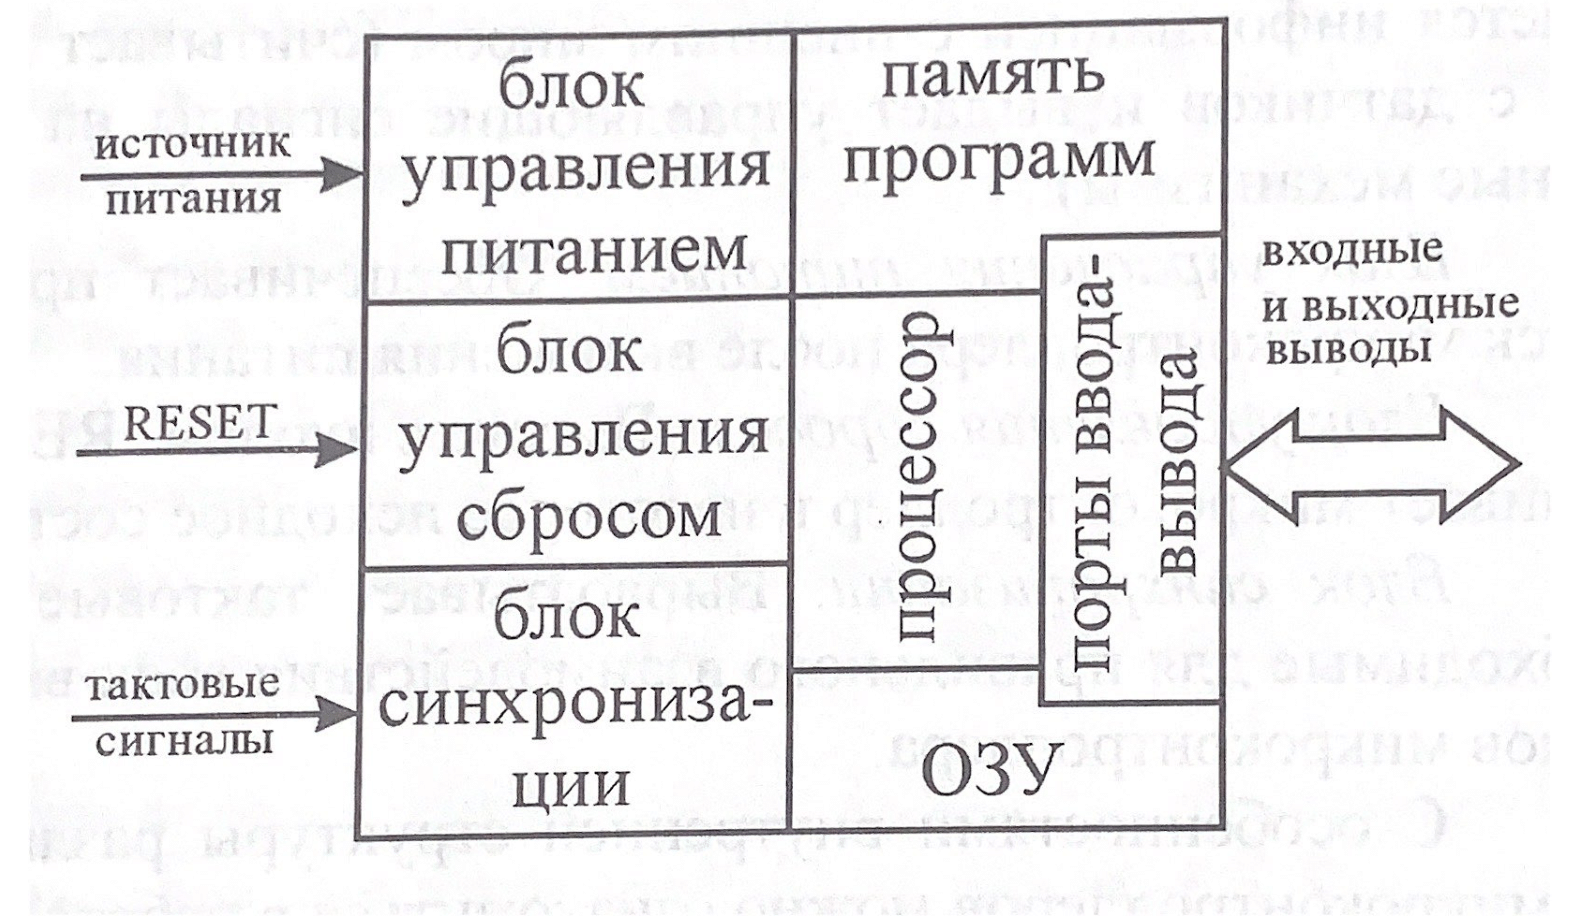
\includegraphics[width=\linewidth]{./src/pics/1.2.1.png}
  \caption{Внутрення структура микроконтроллера.}
  \label{img::1_2_1}
\end{figure}

\begin{itemize}
  \item \textit{Процессор}\\
  Обеспечение обработки информации путём выполнения команды в соответствии 
  с системой команд микроконтроллера.
  \item \textit{Память программ}\\
  Хранение программы, в соответствии с которой работает микроконтроллер.
  \item \textit{ОЗУ}\\
  Другое название ~---~ \textbf{RAM} (Random Access Memory).
  Хранение промежуточных результатов.
  \item \textit{Порты ввода/вывода}\\
  Осуществление обмена информацией с внешним миром.
  \item \textit{Блок управления питанием}\\
  Обеспечение правильности запуска микроконтроллера
  после включения питания.
  \item \textit{Блок управления сбросом}\\
  Установка вместе с входом $RESET$ микроконтроллера в 
  некоторое исходное состояние.
  \item \textit{Блок синхронизации}\\
  Выработка тактовых сигналов, необходимых для правильного взаимодействия 
  всех внутренних блоков микроконтроллера.
\end{itemize}

\subsection{Какие значения записаны в TCCR после сигнала RESET.}
После сигнала $RESET$ все разряды будут установлены в нулевое значение.

\subsection{Порт А. Сколько прерываний и сколько регистров ввода/вывода принадлежит порту А. Назначение этих регистров ввода/вывода.}

Для порта А не предназначено ни одного прерывания. Три регистра: PORTA, DDRA, PINA.
DDRn - на вход или выход работает вывод, PORTn - выходное значение, PINn - входное значение.


\subsection{Регистр SREG. Назначение его  разрядов.}
Регистр $SREG$ ~---~ $8$-разрядный регистр признаков (регистр флагов).
Назначение разрядов приведено на рис. \ref{img::2_3_2}
\begin{figure}[h]
  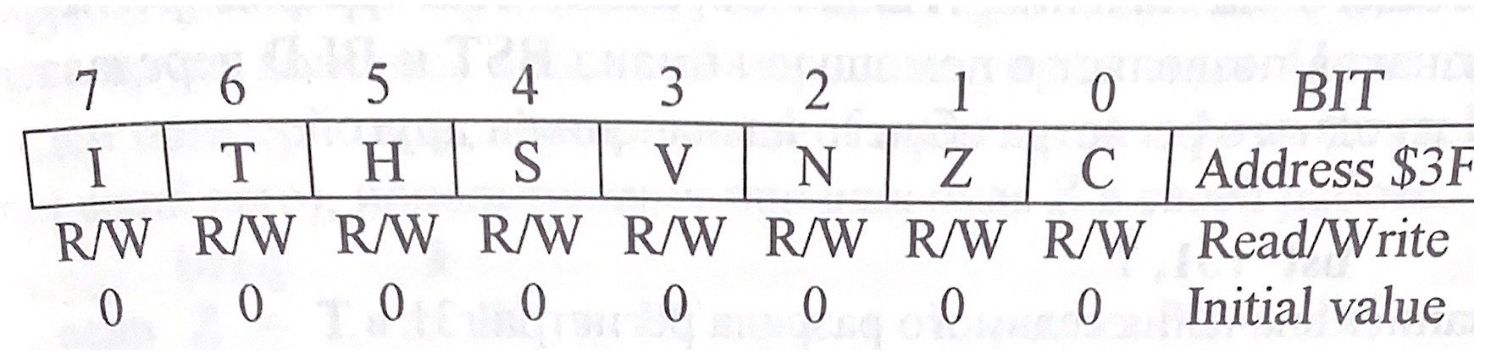
\includegraphics[width=\linewidth]{./src/pics/2.3.2.png}
  \caption{Назначение разрядов регистра $SREG$}
  \label{img::2_3_2}
\end{figure}
Рассмотрим подробнее назначение разрядов:
\begin{itemize}
  \item Бит $7$ -- $I$\\
  Глобальное разрешение прерываний.
  Если в этом разряде нуль, то никакие прерывания не будут обрабатываться.
  Бит обнуляется при возникновении любого прерывания, 
  и автоматически выставляется в единицу при выходе из прерывания.
  \item Бит $6$ -- $T$\\
  Временное хранение бита.
  С помощью команд $BST$ и $BLD$ позволяет передавать
  бит из одного регистра общего назначения в другой. Например,
  следующий код:
  \begin{verbatim}
    bst r31, 7 ; запись значения седьмого разряда регистра r31 в T
    bld r0, 3  ; запись из T в третий разряд регистра r0
  \end{verbatim}
  \item Бит $5$ -- $H$\\
  Признак переноса между полубайтами.
  \item Бит $4$ -- $S$\\
  Равен сумме по модулю $2$ содержимого третьего и второго разряда
  регистра $SREG$.
  \item Бит $3$ -- $V$\\
  Признак переполнения.
  \item Бит $2$ -- $N$\\
  Признак отрицательного результата.
  \item Бит $1$ -- $Z$\\
  Признак нуля.
  \item Бит $0$ -- $C$\\
  Признак переноса.
\end{itemize}

\subsection{Почему после сигнала RESET все прерывания запрещены.}
Для обеспечения корректной инициализации работы
микроконтроллера.

\subsection{Приведите пример использования разряда Т в регистре SREG.}
\begin{verbatim}
  bst r30, 5 ; запись значения пятого разряда регистра r30 в T
\end{verbatim}


\subsection{Таймер 0. Режимы работы, количество прерываний, регистры ввода/вывода, принадлежащие таймеру 0.}

Режимы работы:
\begin{itemize}
  \item Normal (0)\\
  Счётчик $TCNT0$ функционирует как обычный суммирующий счётчик.
  \item PWM Phase Correct (1)\\
  Режим ШИМ с точной фазой. Предназначен для генерации сигналов с 
  широтно-импульсной модуляцией.
  \item CTC -- Clear Timer on Compare match (2)\\
  Режим счёта по модулю, который определяется содержимым регистра $OCR0$.
  \item Fast PWM (3) \\
  Быстродействующий ШИМ. Позволяет генерировать высокочастотный сигнал 
  с широтно-импульсной модуляцией.
\end{itemize}

Прерывания:
\begin{itemize}
  \item $TIMER0\_OVF$ -- переполнение таймера
  \item $TIMER0\_COMP$ -- содержимое счётчика $TCNT0$ совпадает с 
  содержимым регистра $OCR0$.
\end{itemize}

Имеет $3$ регистра ввода-вывода. Ещё $2$ регистра используются совместно 
с таймерами $1$ и $2$:
\begin{itemize}
  \item $TCCR0$ -- Регистр контроля
  \item $SFIOR$ -- Регистр обнуления
  \item $TIMSK$ -- Регистр прерывания
  \item $TIFR$ -- Регистр флагов прерываний
\end{itemize}

Также есть возможность использования двух выводов микроконтроллера:
\begin{itemize}
  \item вход $T0$ ~---~ Timer/Counter0 External Counter Input -- вывод $PB0$
  \item выход $OC0$ ~---~ Timer/Counter0 Output Compare Match Output -- вывод $PB3$
\end{itemize}

\subsection{В каких режимах таймера 0 порог изменяется не сразу (двойная буферизация записи) при записи нового значения в регистр порога с помощью команды OUT. }
\begin{itemize}
  \item PWM Phase Correct (1)\\
Режим ШИМ с точной фазой. Предназначен для генерации сигналов с
широтно-импульсной модуляцией.
  \item Fast PWM (3) \\
Быстродействующий ШИМ. Позволяет генерировать высокочастотный сигнал
с широтно-импульсной модуляцией.
\end{itemize}

\subsection{Откуда приходит сигнал на вход TCNT0.}
Сигналы на вход $TCNT0$ приходят с выхода управляемого предварительного 
делителя частоты.


\subsection{Как можно разрешить (запретить) прерывания по переполнению таймера 0.}
Разрешить:
\begin{verbatim}
  ldi r16, 1 << TOIE0
  out TIMSK, r16
\end{verbatim}

Запретить:
\begin{verbatim}
  ldi r16, 0 << TOIE0
  out TIMSK, r16
\end{verbatim}

\subsection{Написать программу с использованием таймера 0, вырабатывающую симметричное прямоугольное колебание на одном из выходов порта А.}
\begin{verbatim}
#include <avr/io.h>
#include <avr/interrupt.h>

.global TIMER0_COMP_vect
        TIMER0_COMP_vect:
                          in r16, PORTA
                          eor r16, r17
                          out PORTA, r16
                          reti
.global main
        main:
                          sei ; разрешить прерывания

                          sbi DDRA, DDA0 ; PA0 - выход
                          cbi PORTA, PORTA0 ; PA0 = 0

                          ldi r17, 1 << PORTA0
                          ldi r16, 1 << OCIE0 ; разрешить прервание по сарвнению
                          out TIMSK, r16

                          ldi r16, 0x7f ; treshold on half-way
                          out OCR0, r16

                          ldi r16, 1 << WGM00 | 1 << CS00 ; phase-correct PWM
                          out TCCR0, r16

loop:
                          nop
                          nop
                          rjmp loop
\end{verbatim}

\subsection{Какие коэффициенты деления частоты позволяет получать предварительный делитель таймера 0.}
1, 8, 64, 256, 1024

\subsection{Какой режим таймера 0 позволяет вырабатывать треугольные колебания, используя дополнительную интегрирующую цепочку.}
В режимах Normal и CTC --  нужно поставить $OC0$ изменяется при совпадении с порогом.

В ШИМ режимах -- выставить порог в половину максимального.

\subsection{Как запрограммировать предварительный делитель таймера 0.}
В разряды $2:0$ регистра $TCCR0$ записать значение от $1$ до $5$.

\subsection{Режим 0 таймера 0.}
Режим Normal. В этом режиме счётчик $TCNT0$ функционирует как обычный 
суммирующий счётчик. По каждому импульсу тактового сигнала, 
поступающего с выхода предварительного делителя, содержимое
$TCNT0$ увеличивается на единицу. 
При переходе через значение $\$FF$ возникает переполнение, и счёт продолжается
со значения $\$00$. Переполнение вызывает установку в единицу флага переполнения
$TOV0$.

При совпадении значения $TCNT0$ со значением
$OCR0$ флаг прерывания $OCF0$ в регистре $TIFR$ устанавливается в единицу, 
при разрешении прерывание начинает обрабатываться.


\subsection{Режим 1 таймера 0.}
Режим PWM Phase Correct ~---~ режим ШИМ с точной фазой.
Предназначен для генерации сигналов с широтно-импульсной модуляцией. 
$TCNT0$ -- реверсивный счётчик, изменение его состояния 
осуществляется по каждому импульсу тактового сигнала,
поступающего от предварительного делителя. 
Состояние сначала изменяется от $\$00$ до $\$FF$, затем
обратно до $\$00$. При достижении максимального (минимального) 
значения счётчиком, происходит смена направления счёта. 
После достижения значения $\$00$ дополнительно устанавливается 
в единицу флаг прерывания $TOV0$ регистра $TIFR$.

При совпадении значения счётчика $TCNT0$ со значением порога (регистр $OCR0$), 
флаг $OCF0$ выставляется в $1$ и состояние выхода $OC0$ изменяется.

Особенность режима ~---~ двойная буферизация записи в регистр $OCR0$. 
Буферизация заключается в том, что записываемое число на самом деле сохраняется в
специальном буферном регистре.

Изменение содержимого регистра порога происходит после достижения
счётчиком $TCNT0$ максимального значения.

\subsection{Режим 2 таймера 0.}
Режим $CTC$ ~---~ Clear Timer on Compare Match, режим счета по модулю, который определяется 
содержимым регистра $OCR0$. $TCNT0$ обнуляется после того как его содержимое сравняется с 
содержимым регистра $OCR0$. Далее счет продолжается от $\$00$ до нового совпадения с порогом. 
При совпадении содержимого счетчика $TCNT0$ и регистра порога $OCR0$, устанавливается в <<$1$>> 
флаг $OCF0$ и прерывание (если разрешено) начинает обрабатываться.

Счетчик считает от $0$ до $OCR0$. Генерируется прерывание по сравнении и при $OCR0 = 255$ 
полностью совпадающим с режимом $0$

\subsection{Режим 3 таймера 0.}
Режим Fast PWM ~---~ быстродействующий ШИМ. Позволяет генерировать
высокочастотный сигнал с широтно-импульсной модуляцией. Используется 
в регулировании мощности, выпрямлении, цифроаналоговом преобразовании и др.

Значение счётчика $TCNT0$ изменяется от $\$00$ до $\$FF$, после чего 
обнуляется и счёт начинается сначала. 


Особенность режима ~---~ двойная буферизация записи в регистр $OCR0$.
Буферизация заключается в том, что записываемое число на самом деле сохраняется в
специальном буферном регистре.

Изменение содержимого регистра порога происходит после достижения 
счётчиком $TCNT0$ максимального значения. 

\subsection{Когда меняется порог в режиме 3 таймера 0.}
Состояние счетчика $TCNT0$ изменяется от $\$00$ до $\$FF$, после чего он обнуляется и счет 
повторяется. При переходе к состоянию $\$00$ устанавливается флаг прерывания $TOV0$ в 
регистре $TIFR$.

\subsection{Можно ли писать в $TCNT0$ без остановки счета.}

Запись и чтение в $TCNT0$ можно осуществлять без остановки счета.

\subsection{Как можно остановить счет в таймере 0.}


\subsection{Система прерываний микроконтроллера ATmega8535.}


\subsection{Сколько всего прерываний у ATmega8535.}


\subsection{Как организовать вложенные прерывания.}


\subsection{Как можно разрешить (запретить) одновременно все прерывания.}


\subsection{Как организована система приоритетов при обработке прерываний. }


\subsection{Какое минимальное время требуется для преобразования в АЦП.}


\subsection{Чем сигнальный процессор отличается от МК.}


\subsection{Зачем в программе надо устанавливать начальное значение Stack Pointer и чему это значение должно быть равно.}


\subsection{Сторожевой таймер и особенности его работы.}


\subsection{Что такое SPI и зачем он нужен.}


\subsection{Как инициировать передачу байта в SPI.}


\subsection{Сколько прерываний и сколько регистров ввода/вывода принадлежит SPI.}


\subsection{Далее пойдут вопросы про однопроводный интерфейс (сеть MicroLAN).}


\subsection{Сколько проводов необходимо для реализации однопроводного интерфейса.}


\subsection{Как выглядит физический ноль и физическая единица.}


\subsection{Как в однопроводном интерфейсе передается информационный ноль и информационная единица? Какова максимальная скорость  передачи?}

В однопроводном интерфейсе передаются информационный ноль и информационная единица -- 
логически; максимальная скорость  передачи $0$ -- длинный импульс физического нуля ($60$ мкс),
$1$ - короткий ($15$ мкс).

\subsection{Что такое серийный номер в однопроводном интерфейсе и какова его структура.}

Серийный номер в однопроводном интерфейсе -- $64$ бита: $8$ бит -- код семейства, $48$ бит -- 
серийный номер, $8$ бит -- контрольная сумма - уникальный идентификатор устройства, 
чтобы можно было выбрать устройство.

\subsection{Какая команда позволяет Master определить номера всех Slave в сети MicroLAN.}

Search ROM

\subsection{Как выглядит сигнал сброса в сети MicroLAN.}

Сигнал сброса в сети MicroLAN: Долгий импульс нуля ($480$ мкс), потом долгий импульс единицы, 
в течении которой master проверяет, есть ли кто-нибудь в сети.
